\chapter{Low Frequency De-dispersion} \label{appen:low-frequency-dd}

As with all studies of radio transients that emit on sub-second timescales it is important to de-disperse the data to account for smearing caused by propagation through the ISM. Failure to de-disperse causes any observed pulse to broaden and signifcanlty reduce the signal to noise ratio. The dominant factors that cause smearing can be classified in the following `smear budget'.

\begin{equation}
    t_{total\; smear} = \sqrt{\,t_{\mathrm{samp}}^{2} + t_{\mathrm{chan,max}}^{2} + t_{\mathrm{SB}}^{2} + t_{\mathrm{BW}}^{2} + t_{\mathrm{scat}}^{2}\,}
    \label{eq:smear_budget}
\end{equation} 

Here $t_{\text{samp}}$ is the time resolution of the data, in this case $0.655~$ms. $t_{\text{chan}}$ is the intra-channeling smearing which is expressed as, 

\begin{equation}
    t_{chan,i} (\text{DM}, \; f_{\rm top}, \; f_{\rm low}) = \mathcal{D} \cdot \text{DM} \cdot \left( f^{-2}_{\rm low,i} - f^{-2}_{\rm top,i} \right)
\end{equation}

Where $f_{low,i}$ and $f_{top,i}$ are the edge frequencies of a channel. $t_{\mathrm{chan,max}}^{2}$ refers to the max amount of smearing a channel, in this case it's the lowest frequency 110~MHz. The next term is the smearing caused if the data is split into $N$ subbands, the smearing is influenced by the DM error, thus the max smearing that can be caused is when $\Delta \text{DM}/2$

\begin{equation}
    t_{\rm SB} = \mathcal{D} \cdot  \frac{\Delta\text{DM}}{2} \cdot \left( f^{-2}_{\rm low,i} - f^{-2}_{\rm top,i} \right)
\end{equation}

Similarly there is smearing caused by having an incorrect DM value across the entire bandwidth, denoted by $t_{\text{BW}}$ and expressed as, 

\begin{equation}
    t_{\rm BW} = \mathcal{D} \cdot \text{DM} \cdot \left[ \left(f_{\rm low} - \frac{\Delta f}{2}\right)^{-2} -\left(f_{\rm top} - \frac{\Delta f}{2}\right)^{-2}\right]
\end{equation}

Where $\Delta f$ is the frequency resolution of the data, in this case is 0.02~MHz. The final term that needs to be consider is the smearing caused due to scattering which is taken as a relation from \cite{bhat_multifrequency_2004}. 

\begin{equation}
    \text{log} \; t_{scat} = -6.46 + 0.154 \ (\text{log DM}) + 1.07 \ (\text{log DM})^2 - (3.86 \pm 0.16) \log f
\end{equation}

For this survey 600 \dm is chosen as upper limit to for as the smearing is 745.9~ms and scattering becomes the dominant factor at 844.2~ms at 109.9609375~MHz. The individual components of smearing for this survey for the high time resolution data product (.0001) is shown in \cref{fig:DDplan}. 

\begin{figure}
    \centering
    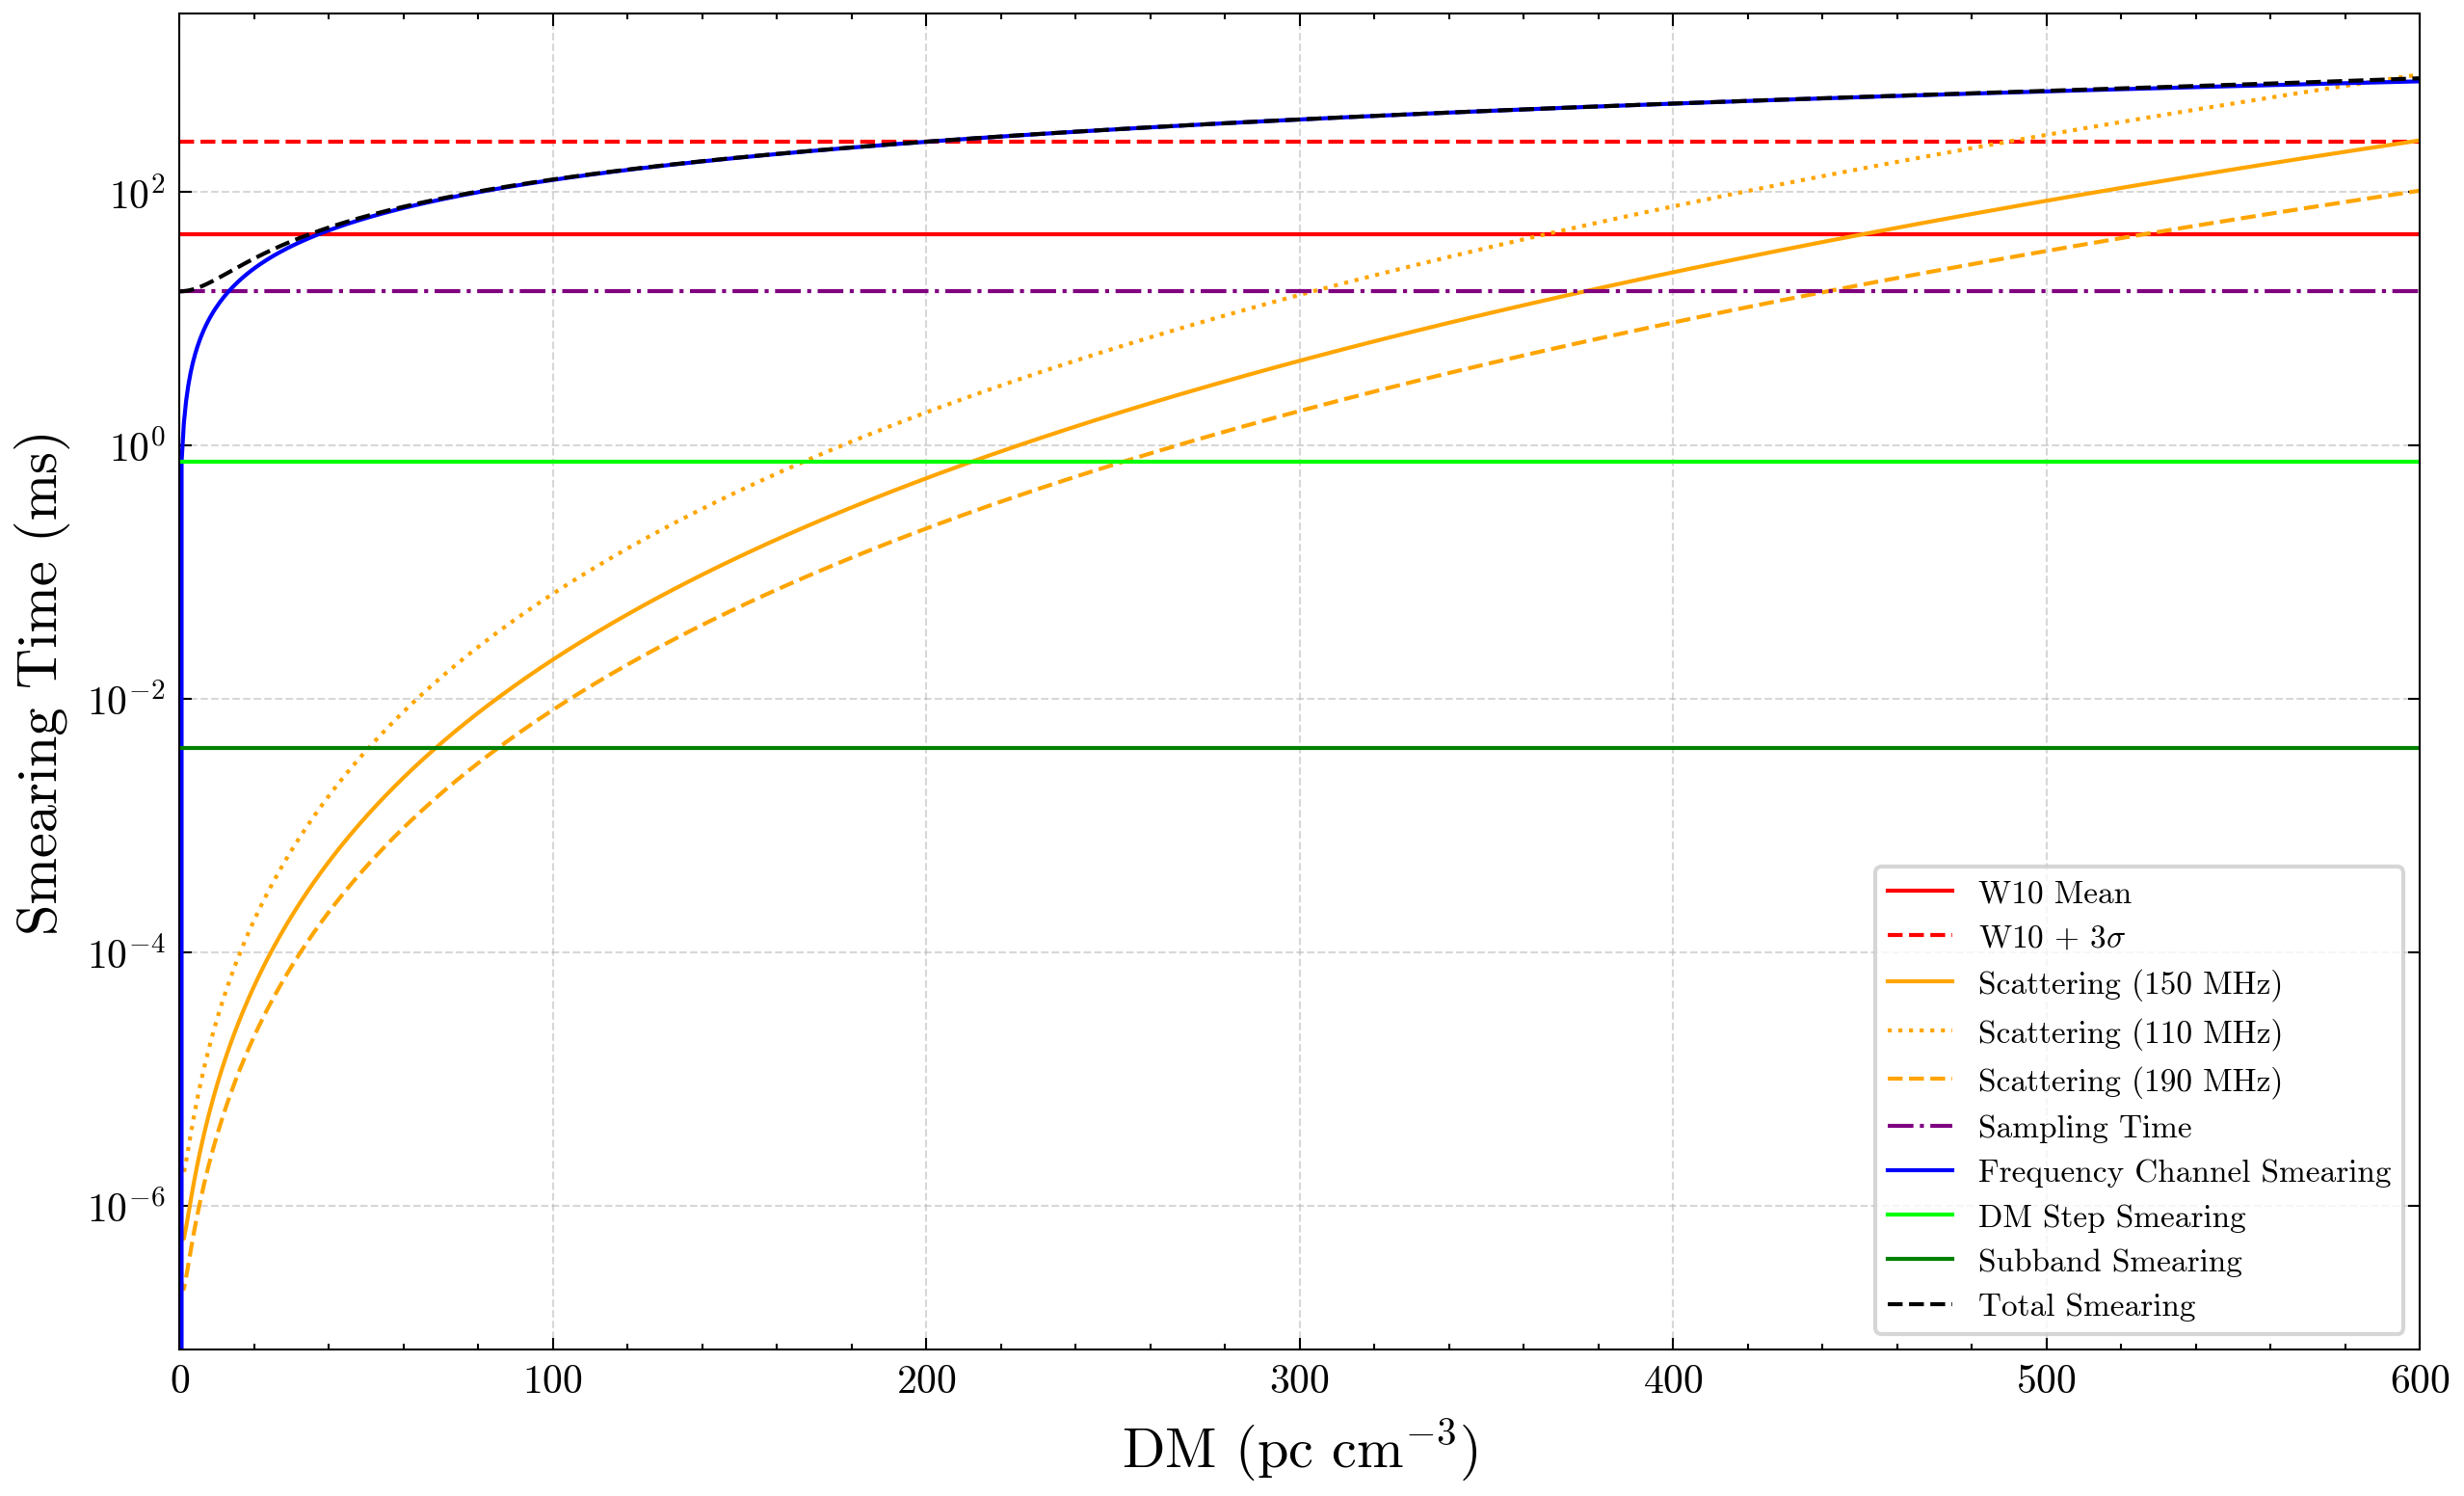
\includegraphics[width=0.9\linewidth]{chapter6/figures/apendicies/ddm_plan_f110-190_dt16.384_df0.2_dm600.png}
    \caption{Smearing due to dispersion measure. Shown is total (black), intra-channel (blue), DM-step (lime), and bandwidth (green) smearing. In red is the the 10\% pulse width values in ms from the ATNF catalogue at the time of writing. Scattering shown at the top, centre and bottom of the band are shown in orange. This was calculated using the observational parameters shown in \cref{tab:frequency_products}.  }
    \label{fig:DDplan}
\end{figure}

\subsection{Optimizing DM Step Values}

To balance residual full-band smearing from the DM grid against the intrinsic channel smearing, let
\begin{equation}
  t_{\rm BW}\bigl(\Delta{\rm DM}\bigr) \;=\; t_{\rm chan,max}({\rm DM}),
\end{equation}
with
\begin{equation}
  t_{\rm chan,max}({\rm DM}) \;=\; \max_i \left\{ \mathcal{D}\,{\rm DM}\,\bigl(f^{-2}_{{\rm low},i}-f^{-2}_{{\rm high},i}\bigr)\right\},
\end{equation}
and the full-band residual from the DM step (worst-case error \(\Delta{\rm DM}/2\))
\begin{equation}
  t_{\rm BW}\bigl(\Delta{\rm DM}\bigr) \;=\; \mathcal{D}\,\frac{\Delta{\rm DM}}{2}\,\bigl(f^{-2}_{\rm low}-f^{-2}_{\rm high}\bigr).
\end{equation}

Solving for the DM step gives

\begin{equation}
  \boxed{\,\Delta{\rm DM}({\rm DM}) \;=\;
  \frac{2\,t_{\rm chan,max}({\rm DM})}{\mathcal{D}\,\bigl(f^{-2}_{\rm low}-f^{-2}_{\rm high}\bigr)}\,}
  \label{eq:ddm_opt}
\end{equation}

substituting gives the following, 

\begin{equation}
  \Delta{\rm DM}({\rm DM}) \;=\;
  \frac{2\,{\rm DM}\;\displaystyle\max_i\!\left(f^{-2}_{{\rm low},i}-f^{-2}_{{\rm high},i}\right)}
       {\,f^{-2}_{\rm low}-f^{-2}_{\rm high}\,}.
\end{equation}

\noindent In practice, trials are generated by starting at ${\rm DM}_0$ and stepping by $\Delta{\rm DM}$ evaluated at the current (or midpoint) DM, yielding a grid that widens with DM.

\begin{table}[h]
    \centering
    \begin{tabular}{cccc}
    \hline \hline 
    DM Start (\dmn)& DM Stop (\dmn) & $\Delta \rm DM$ (\dmn)& Trials $(n)$ \\
    \hline
    0.000   & 0.601   & 0.007  & 92 \\
    0.601   & 2.402   & 0.026  & 69 \\
    2.402   & 7.808   & 0.085  & 64 \\
    7.808   & 25.225  & 0.275  & 64 \\
    25.225  & 79.880  & 0.871  & 63 \\
    79.880  & 252.853 & 2.759  & 63 \\
    252.853 & 600.000 & 6.546  & 54 \\
    \hline
    \end{tabular}
    \caption{DM plan from 0--600 \dm based on the observational setup detailed in \cref{tab:frequency_products} for an international station using the HBA.}
    \label{tab:placeholder}
\end{table}